\documentclass{article}

\usepackage[preprint]{neurips_2020}
% \usepackage[final]{neurips_2020}
% \usepackage[nonatbib]{neurips_2020}

\usepackage[utf8]{inputenc} % allow utf-8 input
\usepackage[T1]{fontenc}    % use 8-bit T1 fonts
\usepackage{hyperref}       % hyperlinks
\usepackage{url}            % simple URL typesetting
\usepackage{booktabs}       % professional-quality tables
\usepackage{amsfonts}       % blackboard math symbols
\usepackage{nicefrac}       % compact symbols for 1/2, etc.
\usepackage{microtype}      % microtypography
\usepackage{graphicx}

\title{Vector Quantized Variational Autoencoders \\on Novel Datasets}

\author{
  Shivanshu Gupta
  \And
  Kolby Nottingham
  \And
  Preethi Seshadri
}

\begin{document}

\maketitle

\begin{abstract}
    We explore using the Vector Quantized Variational Autoencoder (VQ-VAE) to generate discrete representations for the Kaokore dataset, which contains images of facial expressions from traditional Japanese illustrations (\url{https://github.com/rois-codh/kaokore}).
    The framework VQ-VAE is built on, Variational Autoencoders (VAE), learn continuous latent representations.
    While continuous representations are flexible, many real world attributes are better defined discretely, and some current state-of-the art model architectures, like transformers, only work with discrete data. Additionally, VAEs have been shown to exhibit posterior collapse, which means that latent codes are ignored. 
    In this project, we experiment with VQ-VAEs on a novel dataset and design experiments to test the advantages and disadvantages of this approach in terms of generation quality and learned latent structure.
    Since the VQ-VAE paper uses CIFAR10 and 128x128 ImageNet images, there might be additional experimentation and training required to achieve good performance on the Kaokore dataset.
    % VQ-VAEs have been paired with the transformer architecture which, while scalable, can require a lot of compute, so we will experiment with making the method more compute efficient.  % Not sure what to put in this sentence??? Maybe something generic for now.
    We demonstrate the strengths and weaknesses of VQ-VAEs over traditional VAEs. 
\end{abstract}

\section{Introduction}

Generative machine learning models learn...

One such generative machine learning model is the variational autoencoder (VAE). VAEs learn...

While traditional VAEs learn a continuous latent space, vector quantized variational autoencoders (VQ-VAE) learn discrete latent variables. Discrete variables have the advantage when it comes to...

In this work, we compare traditional VAEs to thier discrete counterpart, VQ-VAEs. We implement each of these methods and run experiemnts with each on the Kaokore dataset. To the best of our knowledge, this is the first time VAEs have been used to learn a latent space for this dataset.

\section{Background}

Generative models...

Autoencoders...

\section{Variational Autoencoders}

\section{Vector Quantized Variational Autoencoders}

\section{Experiments}

In a series of experiments, we compare traditional VAEs to VQ-VAEs. We first...

\subsection{Kaokore Dataset}

The Kaokore dataset consists of...

\subsection{Results}

\begin{table}[t]
    \centering
    \begin{tabular}{c c c}
        & Loss & Recon. Loss \\
        \hline
        VAE testset & 0 & 0 \\
        VQ-VAE testset & 0 & 0
    \end{tabular}
    \caption{Training loss and reconstruction loss on the Kaokore testset for both algorithms.}
\end{table}

\begin{figure}[t]
    \centering
    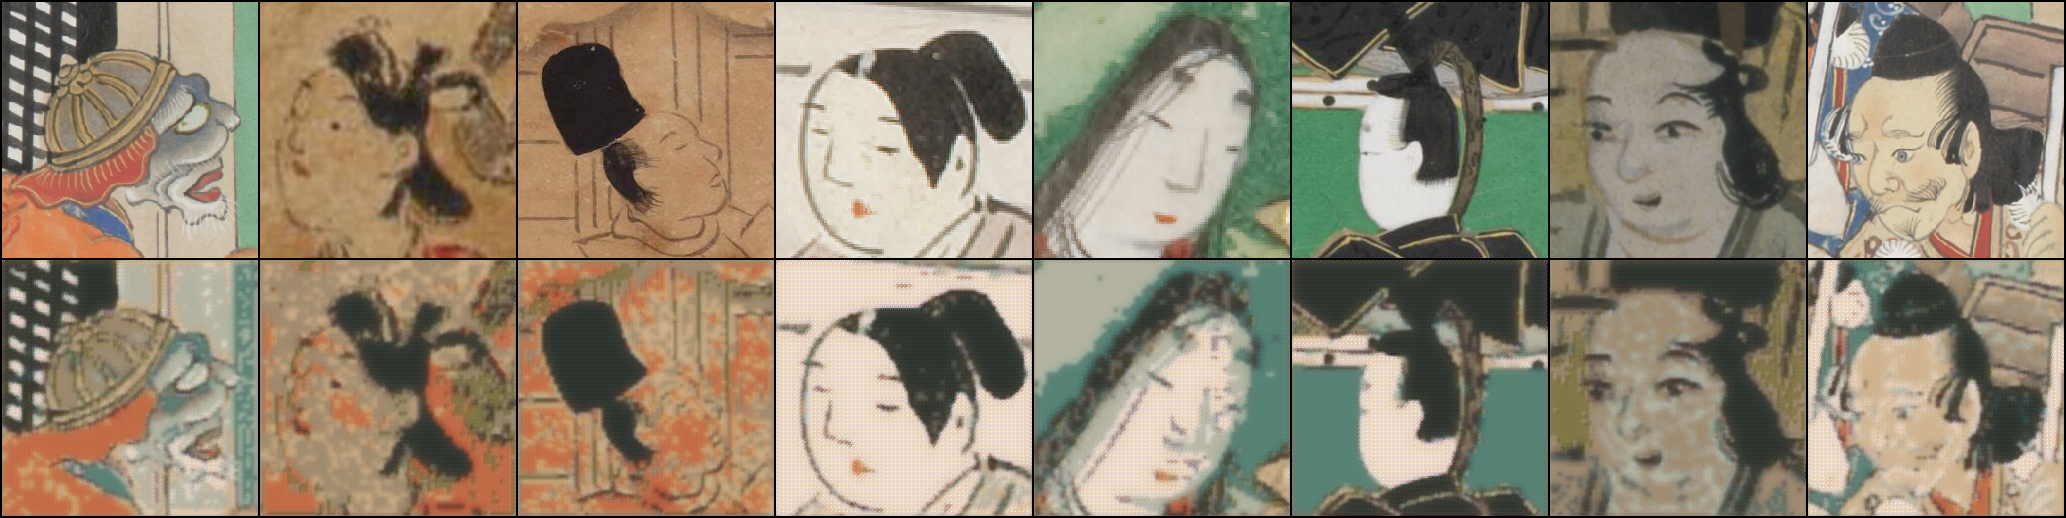
\includegraphics[trim=0 9cm 0 0, clip, width=.8\linewidth]{generation_sample.png}
    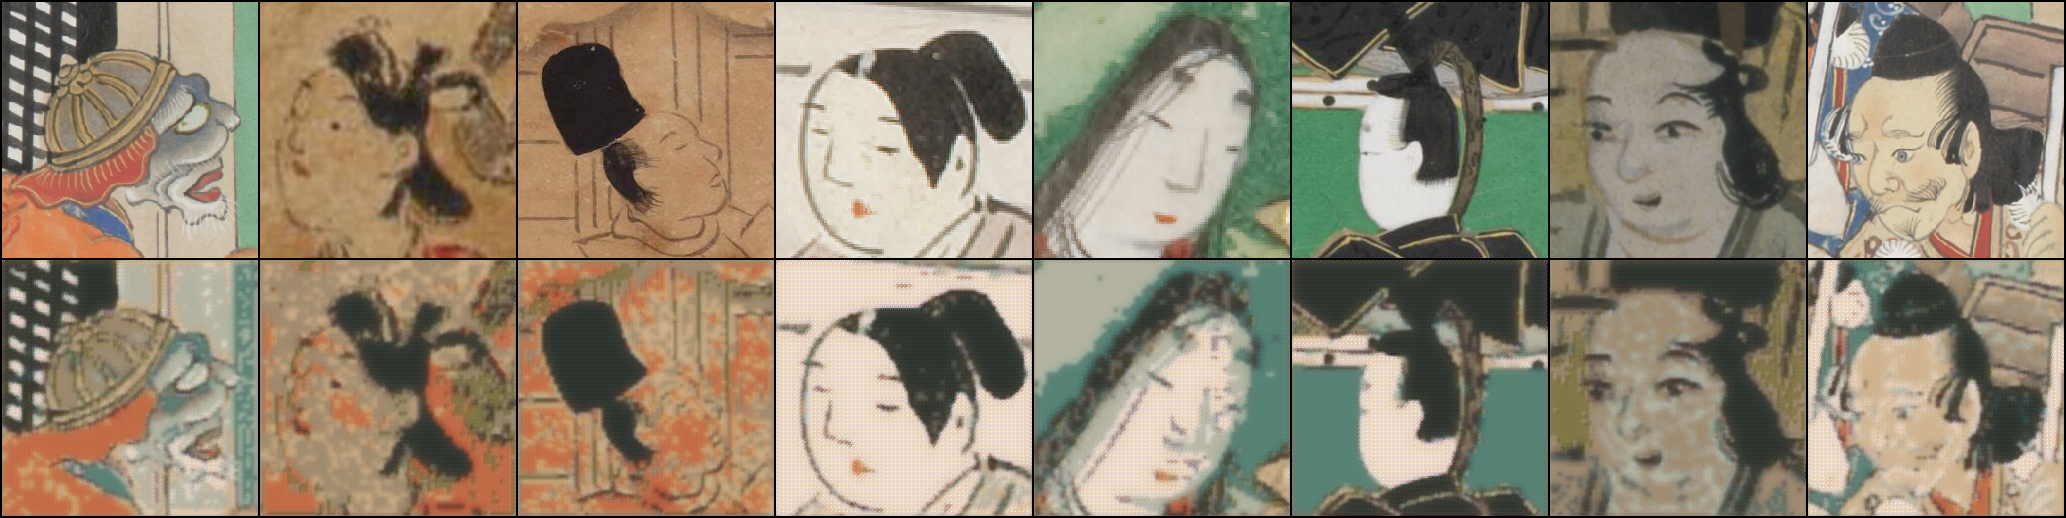
\includegraphics[trim=0 0 0 9cm, clip, width=.8\linewidth]{generation_sample.png}
    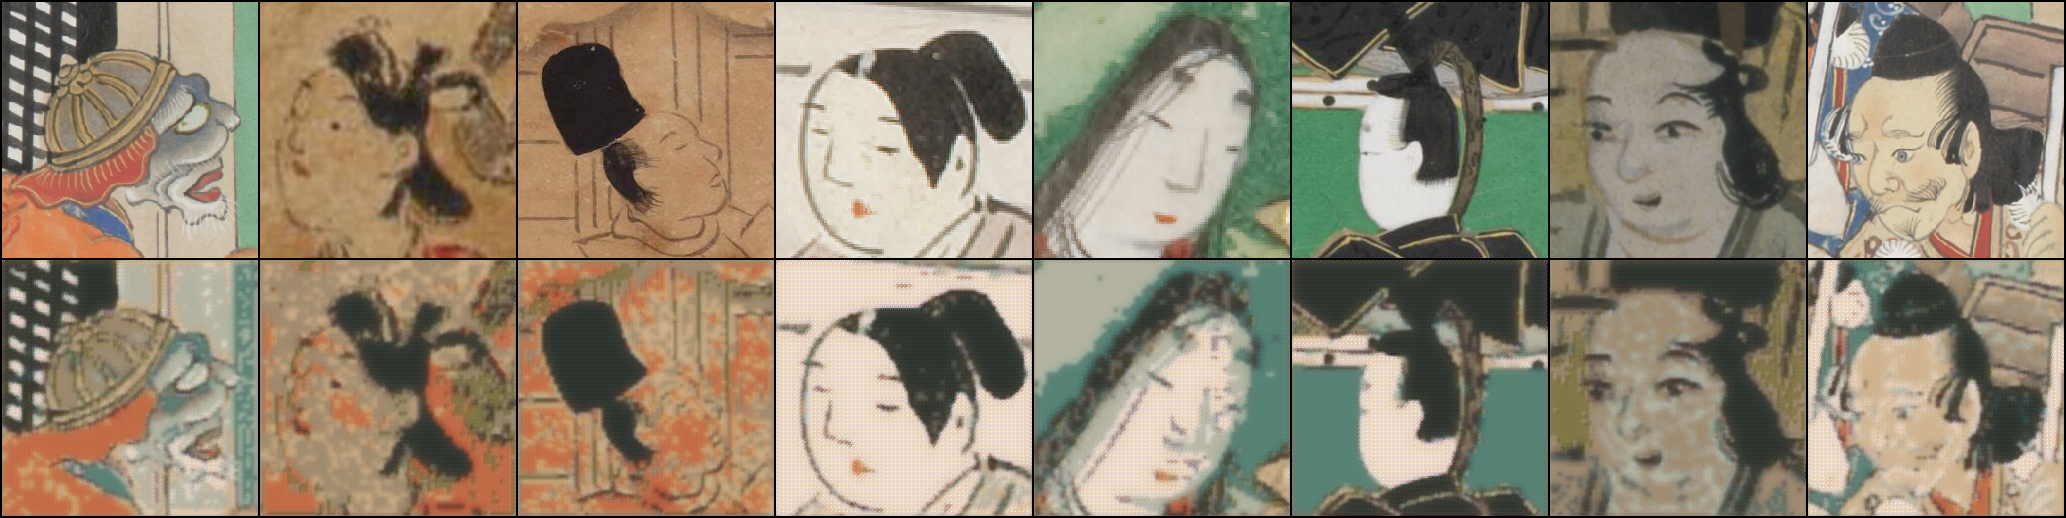
\includegraphics[trim=0 0 0 9cm, clip, width=.8\linewidth]{generation_sample.png}
    \caption{Testset images (top) comared with images generated by VAE (middle) and VQ-VAE (bottom).}
\end{figure}

As indicated in table...

\section{Conclusion}

The authors of the VQ-VAE paper presented promising results. However, bsaed on our experiments, we conclude that it is not strictly better than VAE on every dataset...

\end{document}